\chapter{Resultados}\label{chapter:results}

En este cap\'itulo se presentan los hallazgos clave de nuestro análisis, enfocándose en los resultados relativos a la relación entre el per\'iodo preferido y la excentricidad en diferentes áreas visuales, así como su relevancia en la lateralización hemisférica.

\section{Análisis de la relación entre el tamaño de los pRF y la excentricidad}

\begin{figure}[h]
	\centering
	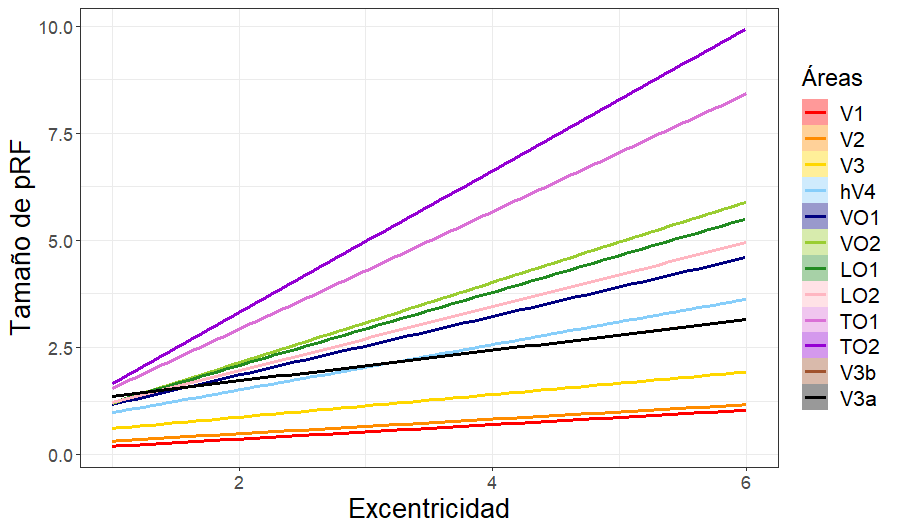
\includegraphics[scale=0.6]{Graphics/size_vs_eccen_bayesian}
	\caption{Gráfico que representa la relación entre el tama\~no de pRF y la excentricidad en las diferentes áreas visuales analizadas.}
	\label{fig:sigma_vs_eccen}
\end{figure}

Aunque no constituye el enfoque principal de este estudio, se llevó a cabo un análisis adicional para examinar la relación entre el tamaño del pRF y la excentricidad en el campo visual. En la Figura \ref{fig:sigma_vs_eccen}, presentamos las rectas de regresión correspondientes a la relaci\'on entre estas variables. Observamos que el tamaño del pRF tiende a incrementarse con la excentricidad, una tendencia que se manifiesta consistentemente a través de las diferentes áreas examinadas. De manera notable, la pendiente de estas rectas de regresión muestra un aumento progresivo al pasar de áreas visuales tempranas, como V1-V3, a áreas de procesamiento visual de nivel superior, tal como TO1. Este hallazgo está en consonancia con investigaciones previas [\cite{wandell_computational_2015}] y refuerza la comprensión de que el tamaño del pRF se expande con la complejidad funcional y jerárquica de las áreas visuales.

\section{Análisis de la relación entre el período preferido y la excentricidad}

En la figura \ref{fig:pp_vs_eccen}, se puede observar que en la mayoría de las áreas visuales analizadas, se cumplen los supuestos de que el período preferido tiende a aumentar con la excentricidad. Sin embargo, es importante destacar que existen variaciones en este patrón.

\begin{figure}[h]
	\centering
	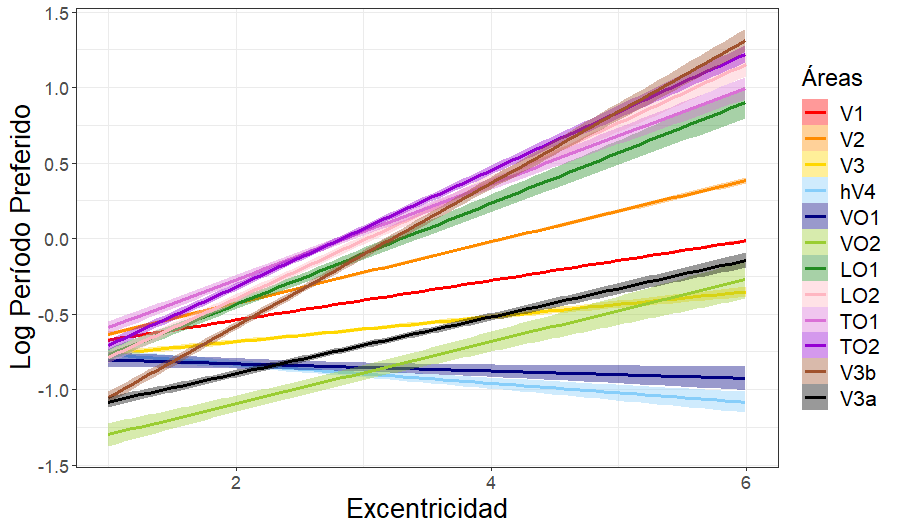
\includegraphics[scale=0.6]{Graphics/pp_vs_eccen}
	\caption{Gráfico que representa la relación entre el logar\'itm del per\'iodo preferido de los v\'oxeles y la excentricidad, en las 12 áreas visuales analizadas.}
	\label{fig:pp_vs_eccen}
\end{figure}

En áreas visuales como hV4 y VO1, se observa una pendiente de crecimiento negativa. Este hallazgo sugiere que, a medida que la excentricidad aumenta, el período preferido tiende a disminuir en lugar de aumentar. Este comportamiento atípico resalta la diversidad de respuestas visuales en diferentes regiones corticales.

Además, en áreas visuales superiores como LO1, LO2, TO1 y TO2,  se evidencia un aumento de la pendiente del período preferido con respecto a la excentricidad, comparado con las áreas visuales tempranas. Esta observación indica que estas áreas específicas muestran un patrón consistente de incremento en el período preferido a medida que nos alejamos del punto central de la visión.

Este análisis proporciona una comprensión más completa de cómo la excentricidad puede modular el período preferido en diversas áreas visuales, destacando la necesidad de considerar la heterogeneidad funcional en la corteza visual.


\section{Resultados del modelo lineal mixto para frecuencias espaciales en función de excentricidad y hemisferio}


En esta secci\'on, se aborda el núcleo central de esta tesis: el análisis del impacto de la frecuencia espacial preferida sobre los hemisferios cerebrales. 

Los resultados obtenidos del modelo lineal mixto \ref{mlm_pp}, aplicado a las frecuencias espaciales de estímulos visuales, se detallan en la Figura \ref{fig:mlm_results_pp}. En esta figura, las filas ilustran las diferentes áreas visuales analizadas mediante el modelo \ref{mlm_pp}, mientras que las columnas, excepto la primera (\'areas), representan las variables fijas con sus respectivos resultados:  estimación de los coeficientes (Coef), error estándar (SE), t-valor (t-val). Adicionalmente, se insert\'o una columna con el factor de Bayes (BF10) con los resultados de la comparaci\'on de cada uno de los modelos propuestos en la secci\'on \ref{mlm}. El BF10 contenido en la columna Excentricidad es resultado de la comparaci\'on del modelo nulo (\ref{m_1}) con el modelo con excentricidad (\ref{m_2}); en la columna Hemisferio de la tabla, se muestra el BF10 de compara los modelos con excentricidad  y con excentricidad y hemisferio (\ref{m_3}) y, en la \'ultima columna se observa el factor BF10 del modelo con excentrididad y hemisferio comparado el modelo \ref{mlm_pp}.


\begin{figure}[h]
	\centering
	
\includegraphics[scale=0.8]{Graphics/table_pp}
	\caption{Tabla que resume los resultados del modelo lineal mixto \ref{mlm_pp} empleado para analizar el per\'iodo preferido de los v\'oxeles en diferentes áreas visuales. Cada fila representa los resultados del modelo para una área visual específica. Para cada variable fija del modelo, la tabla muestra la estimación del coeficiente (Coef), el error estándar (SE) y el valor t (t-val). Además, se incluye el factor de Bayes (BF10) para la comparación entre modelos. El BF10 en la columna 'Excentricidad' corresponde a la comparación entre el modelo \ref{m_1} y \ref{m_2}; en la columna 'Hemisferio', se refiere a la comparación entre el modelo \ref{m_2} y \ref{m_3}; y en la columna 'Excentricidad:Hemisferio', a la comparación entre los modelos \ref{m_3} y \ref{mlm_pp}.}
	\label{fig:mlm_results_pp}
\end{figure}

En el modelo \ref{mlm_pp}, la variable de interés es el periodo preferido, que representa el inverso de la frecuencia espacial. En este modelo, se busca explicar la relación entre el periodo preferido y dos variables independientes: la excentricidad y el hemisferio. Además, se incorporan las diferencias entre sujetos y estímulos para obtener un entendimiento más completo de los factores que influyen en el per\'iodo preferido.

En la Figura \ref{fig:mlm_results_pp}, se aprecia que, con excepción de V01 y hV4, el tamaño del efecto de la excentricidad (Ver Figura \ref{fig:mlm_results_pp}, columna Excentricidad) es mayormente positivo, indicando un aumento en el periodo preferido con la excentricidad. Este hallazgo es respaldado tanto por el valor t como por el factor de Bayes. Además, se observa un patrón consistente de incremento en la magnitud del efecto al pasar de áreas tempranas a aquellas de orden superior, corroborando lo evidenciado en la Figura \ref{fig:pp_vs_eccen}. En el caso de hV4, el coeficiente exhibe un signo negativo y una magnitud inferior en comparación con otras áreas, y es estadísticamente significativo según la prueba t de Student y  el factor de Bayes. Respecto a V01, su coeficiente es notablemente pequeño, y ninguna de las pruebas mencionadas evidencia significancia.

\begin{figure}[h]
	\centering
	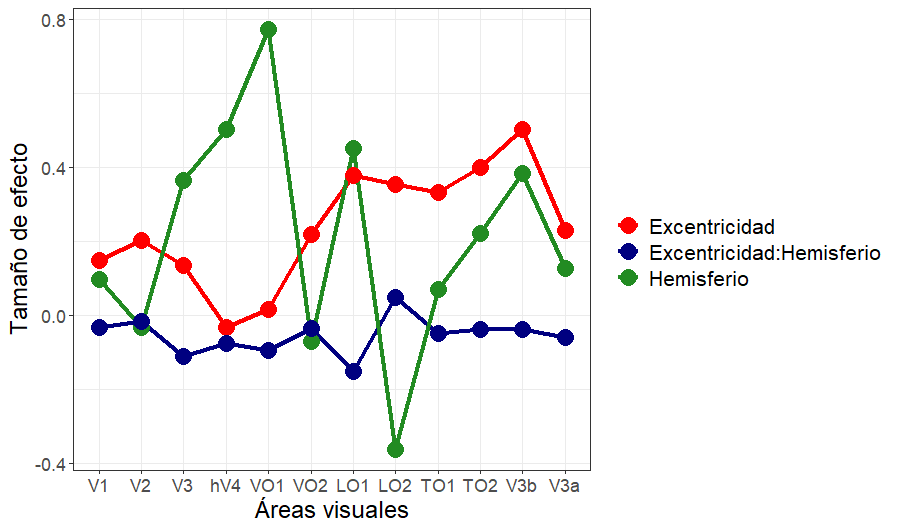
\includegraphics[scale=0.6]{Graphics/effect_size_coef_pp}
	\caption{Representación gráfica de los coeficientes estimados para las variables fijas del modelo lineal mixto \ref{mlm_pp}.}
	\label{fig:coeff}
\end{figure}

Resulta notable que hay un efecto de hemisferio (Ver Figura \ref{fig:mlm_results_pp}, columna Hemisferio) significativo en casi todas las áreas con excepción de V02, pero con coeficientes pequeños en V1, V2, TO1, y V3A . En contraste, las \'areas restantes (V3, hV4, VO1, LO1, LO2, TO2, V3B), presentan coeficientes relativamente grandes (Figura \ref{fig:coeff}), lo cual indica que  el per\'iodo preferido de los v\'ertices corticales en el hemisferio derecho es significativamente mayores que en el izquierdo. Esta diferencia es m\'as pronunciada en las \'areas V01 y hV4 (Ver Figura \ref{fig:hem}). 

Las interacciones entre excentricidad y hemisferio (Ver Figura \ref{fig:mlm_results_pp}, columna Excentricidad:Hemisferio), fueron significativas en varias áreas, pero su magnitud fue relativamente baja en todas las regiones analizadas,

\begin{figure}[h]
	\centering
	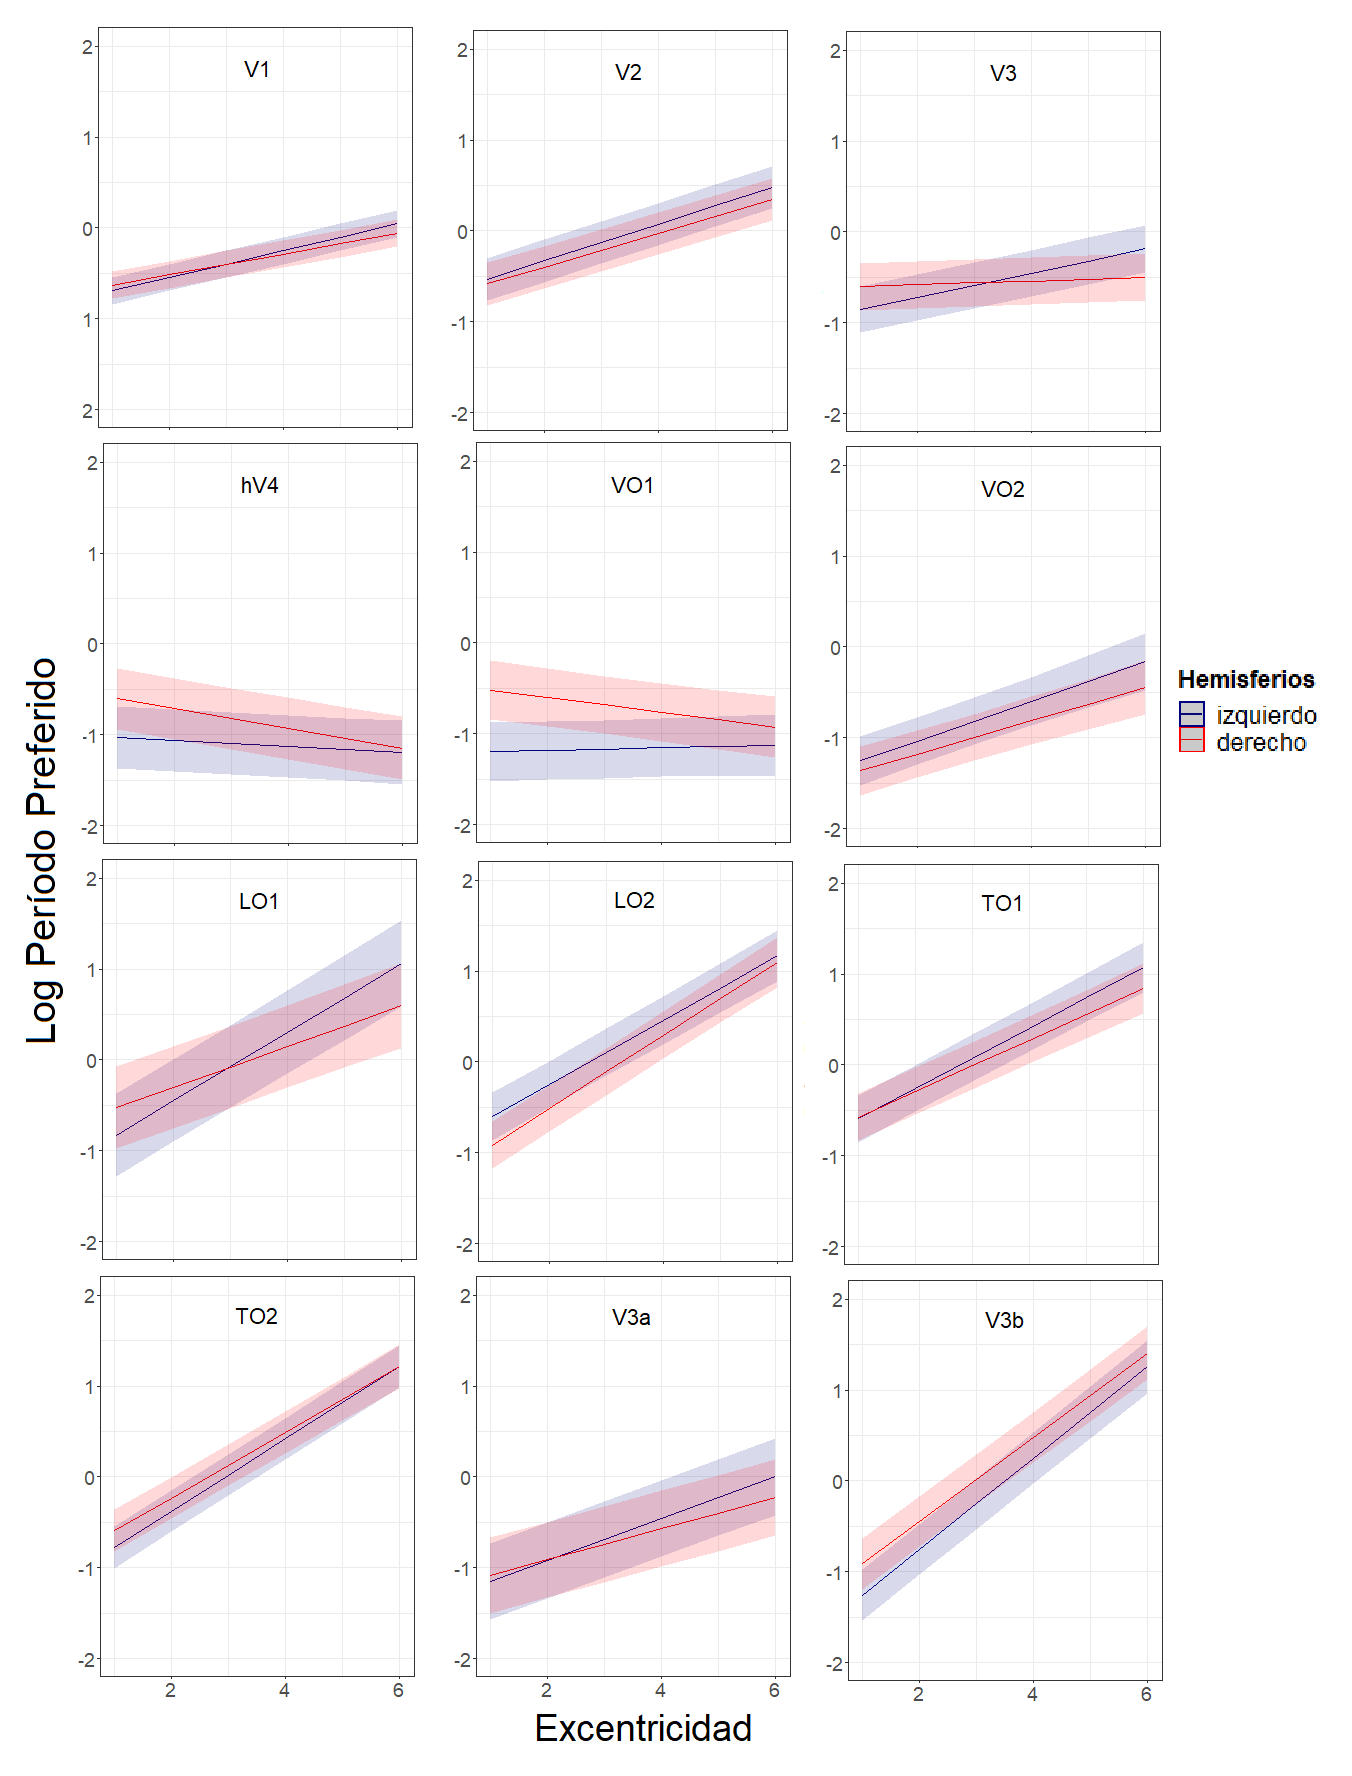
\includegraphics[scale=0.5]{Graphics/compuesto_rois_pp_vs_eccen_hem}
	\caption{Conjunto de gráficas representando la relación entre el logaritmo del per\'iodo preferido de los v\'oxeles y la excentricidad en los dos hemisferios cerebrales, para las 12 áreas visuales analizadas.}
	\label{fig:hem}
\end{figure}













